\documentclass{beamer}

\usepackage[utf8]{inputenc}
\usepackage[brazilian]{babel}

\author{Adriano J. Holanda\\\scriptsize\url{http://adrianoholanda.org/edu}}
\title{Introdução à Computação II\\{\tiny (ou Sistemas Digitais?)}}
\date{7 de agosto de 2013}

\begin{document}

\frame{\titlepage}

\begin{frame}{Objetivos}
  \begin{itemize}[<+-| alert@+>]
  \item Descrever os sistemas numéricos utilizados em circuitos
    digitais, realizando operações aritméticas com números binários.
  \item Caracterizar os circuitos lógicos básicos e suas funções.
  \item Caracterizar lógica combinacional e os circuitos digitais.
  \item Utilizar a álgebra booleana e mapas de Karnaugh para
    simplificação dos circuitos digitais.
  \end{itemize}
\end{frame}

\begin{frame}{Programa}
  \begin{enumerate}[<+-| alert@+>]
  \item Sistemas numéricos
  \item Operações aritméticas com números binários: Adição, Subtração,
    Multiplicação e Divisão
  \item Portas lógicas: {\tt AND}, {\tt OR}, {\tt NAND}, {\tt XOR}
  \item Logica combinacional
  \item Álgebra booleana
  \item Expressões booleanas obtidas a partir de circuitos lógicos
  \item Circuitos lógicos obtidos a partir de expressões booleanas
  \item Tabelas-verdade obtidas a partir de expressões booleanas
  \item Axiomas e teoremas booleanos
  \item Mapas de Karnaugh
  \item Simplificação de circuitos: fatoração e mapas de Karnaugh
  \end{enumerate}
\end{frame}

\begin{frame}{IC2 é pré-requisito para:}
  \begin{itemize}[<+-| alert@+>]
  \item {\small Sistemas Operacionais I e II}
  \item {\Large Introdução à Organização de Computadores}
  \item {\large Algoritmos e Programação de Computadores}
  \end{itemize}
\end{frame}

\begin{frame}{Avaliação}
  \begin{itemize}
  \item 2 Provas: 70\%
  \item 2 Trabalho(s) ou Teste(s): 30\%
  \end{itemize}
  
 Cálculo da nota final (NF)\\

 $$ \text{NF} = 0,7\times \text{m\'edia}(P_1,P_2) + 0,3\times \text{m\'edia}(T_1,T_2)$$
 $$\text{m\'edia}(X_1,X_2) = \frac{X_1+X_2}{2} $$

\end{frame}

\begin{frame}{Bibliografia}
  \begin{thebibliography}{5}
  \bibitem[Tocci]{Tocci,2005}
    Tocci, R. J; Widmer, N. S. 
    \newblock Sistemas digitais: princípios e aplicações. 
    \newblock 8a. edição, São Paulo, Pearson, 2005.

  \end{thebibliography}
\end{frame}

\end{document}
\documentclass{beamer}

\def\classnumber{1} % 0 and 1

\usepackage[brazilian]{babel}
\usepackage{tikz}
\usepackage[utf8]{inputenc}
\usepackage[brazilian]{babel}

\hyphenation{dis-po-si-ti-vos}

\def\slidetransition#1{\frame{\title{#1}\author{}\institute{}\date{}\titlepage}}

%%%%%%%%%%%%%%%%%%%%%%%%%%%%%%%% AULA
%%%%%%%%%%%%%%%%%%%%%%%%%%%%%%%% 1 %%%%%%%%%%%%%%%%%%%%%%%%%%%%%%%%
\if\classnumber=0

\def\thetitle{Conversão de Bases e Aritm\'etica Bin\'aria}

\title{\thetitle}
  
\author{Adriano de Jesus Holanda\\{\scriptsize\url{http://adrianoholanda.org/edu}}}
\institute[]{FAFRAM}
\date{14 de agosto de 2013}

\begin{document}

\frame{\titlepage}

\part{\thetitle}

\frame{\frametitle{Trilha}\tableofcontents[part=1]}

\section{Conversão decimal $\rightarrow$ binário}

\subsection{Representação de inteiros}


\begin{frame}
  \frametitle{Representação de inteiros}

Um {\em byte} pode representar os numeros de 0 a 255 da seguinte forma,\\
\begin{center}
    \begin{tabular}{lll}
      00000000 & = & 0 \\
      00000001 & = & 1 \\
      00101001 & = & 41 \\
      10000000 & = & 128 \\
      11111111 & = & 255 \\
    \end{tabular}
  \end{center}
  
\pause
 Um valor inteiro $A$ de uma sequência de n bits de dígitos binários
 $a_{n-1}a_{n-2}\ldots a_1a_0$ pode ser obtido pela seguinte fórmula:
 \begin{equation}
   \label{eq:magnitudesinal}
   A = \sum_{i=0}^{n-1}2^ia_i
 \end{equation}

\end{frame}

\def\thetitle{Representação em sinal-magnitude}

\subsection{\thetitle}

\slidetransition{\thetitle}

\begin{frame}{\thetitle}

O bit mais significativo (mais à esquerda) representa o \alert{sinal} e o
restante, a \alert{magnitude}.

\begin{center}  
  \begin{tabular}{lll}
    +18 & = & 00010010 \\
    \alert{--}18 & = & \alert{1}0010010 (sinal-magnitude)\\
  \end{tabular}
\end{center}  

O valor do inteiro $A$ é calculado da seguinte forma:\\

\pause
\begin{equation}
  \label{eq:sinalmagnitudemenos}
  A = 
  \begin{cases}
    \displaystyle\sum_{i=0}^{n-1}2^ia_i & \text{se}\ a_{n-1}=0\\
    -\displaystyle\sum_{i=0}^{n-1}2^ia_i & \text{if}\ a_{n-1}=1\\
  \end{cases}
\end{equation}

\end{frame}

\def\binexercise#1{
\begin{frame}{Exercícios}
  Converta os númeiros binários a seguir, admitindo que 
estão na representação~#1, para a base decimal:
\bigskip
\begin{enumerate}
\item {\tt 10110
\item 011011
\item 000110
\item 10010101
\item 100000
\item 101010
\item 010010
\item 100111}
\end{enumerate}
\end{frame}
}

\binexercise{\alert{sinal-magnitude}}

\def\thetitle{Representação em complemento de dois}

\subsection{\thetitle}

\slidetransition{\thetitle}

\begin{frame}{Círculo numérico de quatro bits}

\input{../fig/4bits-circle}

\end{frame}

\begin{frame}{\thetitle}
\begin{center}
  \begin{tikzpicture}
    \tikzset{cell/.style={minimum width=1cm,minimum height=0.5cm,rectangle,draw}}
    \foreach \x/\m/\bin in {0/-128/1,1/64/0,2/32/0,3/16/0,4/8/0,5/4/0,6/2/1,7/1/1} {
      \node[cell,fill=blue,font=\color{white}] at (\x,0) {\m};
      \node[cell] at (\x,-.5) {\only<2->{\bin}};
    }
    \node<3-> at (0,-1) {$-128$};
    \node<3-> at (6,-1) {$+2$};    
    \node<3-> (less) at (7,-1) {$+1$};
    \node<3-> (eq) [right of=less] {$=$};
    \node<3-> [right of=eq] {$-125$};
  \end{tikzpicture}
\end{center}

\only<4>{
\begin{equation}
  \label{eq:sinalmagnitudemenos}
  A = -2^{n-1}a_{n-1} + \displaystyle\sum_{i=0}^{n-2}2^ia_i
\end{equation}
}

\end{frame}

\binexercise{\alert{em complemento de dois}}

\section{Conversão decimal $\rightarrow$ binário}
\footnotesize
\begin{frame}{Conversão base decimal para a binária}
  Outra técnica de conversão utiliza divisões sucessivas por $2$.
  Após as divisões são feitas as escritas, de modo inverso, de cada
  divisão, até que um quociente $0$ seja obtido.
  
    \begin{center}
      \begin{tikzpicture}
        \tikzset{res/.style={fill=gray!40}}
        \foreach \i/\num/\res/\rest in {0/25/12/1,1/12/6/0,2/6/3/0,3/3/1/1,4/1/0/1} {
          \node at (1.*\i,-\i) {${\num\over 2}$};
          \node at (1+1.*\i,-\i) {${=\res}$};
          \node[fill=gray!40] at (1.*\i,-6) {${\rest}$};
          \path[->,draw,>=latex] (1.*\i,-\i-0.35) -- node[rotate=90,above]{resto}  (1.*\i,-5.65);
        }
        \node at (8,-6) {$\Rightarrow \text{inverte a sequência} \Rightarrow 11001 =\ 25_{10}$};
      \end{tikzpicture}
    \end{center}
  \end{frame}


\begin{frame}{Exercícios}
  Converta os seguintes números da base binária para a base decimal:
\bigskip
\begin{enumerate}
\item $34$
\item $52$
\item $29$
\item $45$
\item $11$
\item $189$
\end{enumerate}

\end{frame}

\section{Operações binárias}

\subsection{Lógica}

\subsubsection{Negação}

\begin{frame}{Negação}{Complemento de dois}

  \begin{tabbing}
    $\alert{+}18$  $\rightarrow$ \hspace{3cm} \= $00010010$ \\
    {\small complemento bit a bit}  $\rightarrow$ \> $111011$\=$01$ \\
      \>$+$ \> $1$ \\
       \> $\overline{11101110}$ $=-18$\\
  \end{tabbing}

\pause
  \begin{tabbing}
    $\alert{-}18$  $\rightarrow$ \hspace{3cm}  \= $111011$\=$10$ \\
    {\small complemento bit a bit} $\rightarrow$ \> $00010001$ \\
    \>$+$ \> $1$ \\
    \> $\overline{00010010}$ $=+18$\\
  \end{tabbing}

\end{frame}

\end{document}

\else

%%%%%%%%%%%%%%%%%%%%%%%%%%%%%%%% AULA
%%%%%%%%%%%%%%%%%%%%%%%%%%%%%%%% 2 %%%%%%%%%%%%%%%%%%%%%%%%%%%%%%%%

\begin{document}

\def\thetitle{Aritm\'etica Bin\'aria}
\title{\thetitle}\author{Adriano J. Holanda}\date{21 de agosto de 2013}
\frame{\maketitle}

\section{\thetitle}

\subsection{Adição}

\begin{frame}{Adição}{Complemento de dois}

\begin{columns}
\begin{column}{.3\textwidth}
  \begin{tabular}{rcl}
      $1001$ & = & $-7$ \\
      $+\ 0101$ & = & $5$ \\\hline
      $1110$ & = & $-2$ \\
     \end{tabular}
   \end{column}

\begin{column}{.3\textwidth}
  \begin{tabular}{rcl}
      $1100$ & = & $-4$ \\
      $+\ 0100$ & = & $4$ \\\hline
      ${\color{gray}1}0000$ & = & $0$ \\
     \end{tabular}
   \end{column}
 \end{columns}

\pause
\bigskip
{\color{gray}\hrule}
\bigskip
\begin{columns}
\begin{column}{.3\textwidth}
  \begin{tabular}{rcl}
      $0011$ & = & $3$ \\
      $+\ 0100$ & = & $4$ \\\hline
      $0111$ & = & $7$ \\
     \end{tabular}
   \end{column}

\begin{column}{.3\textwidth}
  \begin{tabular}{rcl}
      $1100$ & = & $-4$ \\
      $+\ 1111$ & = & $-1$ \\\hline
      ${\color{gray}1}1011$ & = & $-5$ \\
     \end{tabular}
   \end{column}

\end{columns}

\pause
\bigskip
{\color{gray}\hrule}
\bigskip
\begin{columns}
\begin{column}{.3\textwidth}
  \begin{tabular}{rcl}
      $\alert{0}101$ & = & $5$ \\
      $+\ \alert{0}100$ & = & $4$ \\\hline
      $\alert{1}001$ & = & \alert{\tt Overflow} \\
     \end{tabular}
   \end{column}

\begin{column}{.3\textwidth}
  \begin{tabular}{rcl}
      $\alert{1}001$ & = & $-7$ \\
      $+\ \alert{1}010$ & = & $-6$ \\\hline
      $\alert{0}011$ & = & \alert{\tt Overflow} \\
     \end{tabular}
   \end{column}


\end{columns}

\end{frame}

\def\thetitle{Subtração}

\subsection{\thetitle}

\begin{frame}{\thetitle}
\begin{center}
  \begin{tikzpicture}
    \tikzset{cell/.style={minimum width=1cm,minimum height=0.5cm}}
    \foreach \x/\s/\m/\c/\r/\rf in {0/0/0/1/0/0,1/1/0/1/0/0,2/0/1/0/1/1,3/1/0/1/0/1} {
      \node[cell] at (\x,0) {\s};
      \node[cell] at (\x,-.5) {\only<1>{\m}\only<2->{\color{red}\c}};
      \node[cell] at (\x,-1.5) {\only<3->{\r}};
      \node[cell] at (\x,-3) {\only<5>{\rf}};
    }
    \node at (4,0) {$\equiv\ 5$};
    \node<1> at (6,0) {\small subtraendo};
    \node<1> at (3.80,-.5) {$\equiv$};
    \node (two) at (4.25,-.5) {$2$};
    \node<1> at (6,-.5) {\small minuendo};
    \node at (-.5,-.5) {\only<1>{$-$}\only<2->{\color{red}$+$}};
    \node<2-> [right of=two,anchor=west] {\small \color{red}
      complemento bit a bit};
    \draw (-.5,-1) -- (3.5,-1);
    \node at (-1,-1.5) {\only<3>{$1$}};
    \node<4-> at (3,-2) {$1$};
    \node<4-> at (-.5,-2) {$+$};
    \draw<4-> (-.5,-2.5) -- (3.5,-2.5);
    \node<5> at (4,-3) {$\equiv\ 3$};
  \end{tikzpicture}
\end{center}

\end{frame}


\def\thetitle{Multiplicação}

\subsection{Multiplicação}

\begin{frame}{\thetitle}
\begin{center}
  \begin{tikzpicture}
    \tikzset{cell/.style={minimum width=1cm,minimum height=0.5cm}}
    \foreach \x/\s/\m/\c/\pa/\pb in {0/0/{\color<5>{red}0}/0/0/0,1/1/{\color<4>{red}0}/0/0/1,2/0/{\color<3>{red}1}/1/0/0,3/1/{\color<2>{red}0}/0/0/1} {
      \node[cell] at (\x,0) {\s};
      \node[cell] at (\x,-.5) {\m};
      \node<2->[cell] at (\x,-1.5) {\pa};
      \node<3->[cell] at (\x-1,-2) {\pb};
      \node<4->[cell] at (\x-2,-2.5) {\pa};
      \node<5->[cell] at (\x-3,-3) {\pa};
      \node<6->[cell] at (\x-1,-4) {\pb};
    }
    \node at (4,0) {$\equiv\ 5$};
    \node<1> at (6,0) {\small multiplicando};
    \node at (4,-.5) {$\equiv\ 2$};
    \node<1> at (6,-.5) {\small multiplicador};
    \node at (-.5,-.5) {$\times$};
    \draw (-3.5,-1) -- (3.5,-1);
    \node<6-> at (-3.5,-3) {$+$};
    \draw<5-> (-3.5,-3.5) -- (3.5,-3.5);
    \foreach \x in {4,-1,-2} {
      \node<6->[cell] at (\x-1,-4) {$0$};
    }
    \node<6> at (4,-4) {$\equiv\ 10$};
  \end{tikzpicture}
\end{center}

\end{frame}

\subsection{Exercícios}

\begin{frame}{Exercícios}
  \footnotesize
  \begin{enumerate}
  \item Represente os seguintes valores de complemento de 2 em
    decimal: 
    \begin{itemize}
      \item 1101011
      \item 0101101
      \end{itemize}
    \item Suponha que os números sejam representados por complemento
      de 2 com 6 bits. Realize a adição binária mostrando todos os
      passos intermediários:
    \begin{itemize}
      \begin{minipage}{.35\textwidth}
      \item $6+13$
      \item $5+21$
      \end{minipage}
      \begin{minipage}{.35\textwidth}
      \item $9+17$
      \item $5+2$
      \end{minipage}
  \end{itemize}
\item Realize as seguintes subtrações binárias (complemento de 2)
  utilizando 4 bits e mostrando os passos intermediários:
    \begin{itemize}
      \begin{minipage}{.35\textwidth}
      \item $8-4$
      \item $9-2$
      \item $6-(-2)$
      \item $2-2$
      \end{minipage}
      \begin{minipage}{.35\textwidth}
      \item $-3-2$
      \item $-3-(-2)$
      \item $8-7$
      \item $7-8$
      \end{minipage}
    \end{itemize}
    \item Realize as seguintes multiplicações, com extensão para 8
      bits no resultado:
      \begin{itemize}
      \item $3\times 4$
      \item $2 \times 3$
      \end{itemize}
    \end{enumerate}
  

\end{frame}

\section{Tabela de conversão de bases}

\begin{frame}{Tabela de conversão decimal, hexadecimal, octal, binário.}
\small

\begin{columns}
  \begin{column}{.5\textwidth}
    
    \begin{tabular}{cccc}\hline
      \bf Dec& 	\bf Hex& 	\bf Oct &	\bf Bin \\\hline
      000&	00&	000&	00000000\\
      001&	01&	001&	00000001\\
      002&	02&	002&	00000010\\
      003&	03&	003&	00000011\\
      004&	04&	004&	00000100\\
      005&	05&	005&	00000101\\
      006&	06&	006&	00000110\\
      007&	07&	007&	00000111\\
      008&	08&	010&	00001000\\
      009&	09&	011&	00001001\\
      010&	0A&	012&	00001010\\
      011&	0B&	013&	00001011\\
      012&	0C&	014&	00001100\\
      013&	0D&	015&	00001101\\
      014&	0E&	016&	00001110\\
      015&	0F&	017&	00001111\\\hline
    \end{tabular}

  \end{column}

  \begin{column}{.5\textwidth}
    \begin{tabular}{cccc}\hline
      \bf Dec& \bf 	Hex &\bf	Oct &\bf	Bin\\\hline
      016&	10&	020&	00010000\\
      017&	11&	021&	00010001\\
      018&	12&	022&	00010010\\
      019&	13&	023&	00010011\\
      020&	14&	024&	00010100\\
      021&	15&	025&	00010101\\
      022&	16&	026&	00010110\\
      023&	17&	027&	00010111\\
      024&	18&	030&	00011000\\
      025&	19&	031&	00011001\\
      026&	1A&	032&	00011010\\
      027&	1B&	033&	00011011\\
      028&	1C&	034&	00011100\\
      029&	1D&	035&	00011101\\
      030&	1E&	036&	00011110\\
      031&	1F&	037&	00011111\\\hline
    \end{tabular}
  \end{column}
\end{columns}
\end{frame}

\end{document}

\fi
\input{00header}

\title{Portas lógicas e circuitos combinacionais}
\author{Adriano J. Holanda}
\date{\today}

\def\OR{{\tt OR}}
\def\AND{{\tt AND}}
\def\NOT{{\tt NOT}}
\def\XOR{{\tt XOR}}

\frame{\maketitle}

\def\mysection{Portas lógicas}

\section{\mysection}


\foreach \GATE/\gate in {\OR/or, \AND/and, \NOT/not, \XOR/xor} {
  
  \begin{frame}{Porta \GATE}
    
    \input{../fig/\gate}
    
  \end{frame}

}

\begin{frame}{Multiplexador (seletor)}

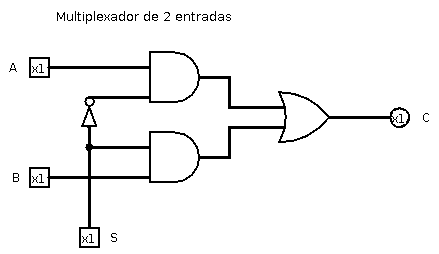
\includegraphics[scale=.6]{../fig/2gates-mux2.png}                            

\end{frame}

\input{zzfooter}

%%% Local Variables:
%%% mode: latex
%%% TeX-master: t
%%% End:


\documentclass{beamer}

\usepackage{standalone}
\usepackage[brazil]{babel}
\usepackage[utf8]{inputenc}

\usepackage{tikz}
\usetikzlibrary{matrix,shapes.gates.logic.US,shapes}
\usepackage{circuitikz}

\title{Circuitos Combinacionais}
\author{Adriano J. Holanda}
\date{9 de novembro de 2013}

\def\AXIOM{{\color{gray}\tt\scriptsize [axioma]}}
\def\THEOREM{{\color{gray}\tt\scriptsize [teorema]}}
\def\NOT#1{{\overline{#1}}}
\def\A{\node{A};}
\def\B{\node{B};}
\def\S{\node{S};}
\def\O{\node{0};}
\def\I{\node{1};}
\colorlet{out}{red}

\begin{document}
\maketitle

\section{Circuitos Lógicos Combinacionais}

\subsection{Álgebra Booleana}

\begin{frame}{Álgebra Booleana}
\footnotesize
Há vários axiomas e teoremas da álgebra booleana que ajudam a manipular 
equações lógicas:

\begin{enumerate}
\item {\bf Identidade}: $A+0=A$ e $A.1=A$; \AXIOM
\item {\bf Inverso}: $A+\NOT{A}=1$ e $A.\NOT{A}=1$; \AXIOM
\item {\bf Comutativo}: $A+B=B+A$ e $A.B=B.A$; \AXIOM
\item {\bf Associativo}: $A+(B+C)=(A+B)+C$ e $A.(B.C)= (A.B).C$; \THEOREM
\item {\bf Distributivo}: $A.(B+C) = (A+B).(A+C)$ e $A+(B.C) = (A+B).(A+C)$;
  \AXIOM
\item {\bf Absorção}: $A+(A.B)=A$ e $A.(A+B)=A$; \THEOREM
\item {\bf De Morgan}: $\NOT{A.B} = \NOT{A} + \NOT{B}$ e
  $\NOT{A+B}=\NOT{A}.\NOT{B}$; \THEOREM
\item {\bf Involução}: $\NOT{\NOT{A}}=A$; \THEOREM
\item $A+A=A$ e $A.A=A$. \THEOREM
\end{enumerate}

\end{frame}

\frame{\centering{\bf\Large Lógica Digital: Circuitos Básicos}}

\subsection{Portas Lógicas}

\begin{frame}[fragile]{Portas Lógicas}
\def\shift{2cm}
\tikzset{every node/.style={font=\scriptsize}}

\begin{circuitikz}
\draw (0,0) node[and port] (AND) {};
\node [above of=AND,xshift=-.45*\shift] {\tt AND};
\node [below of=AND,xshift=-.45*\shift] {\tt $S=A.B$};

\draw (1.5*\shift,0) node[or port] (OR) {};
\node [above of=OR,xshift=-.45*\shift] {\tt OR};
\node [below of=OR,xshift=-.45*\shift] {\tt $S=A+B$};

\draw (2.5*\shift,0) node[not port] (NOT) {};
\node [above of=NOT,xshift=-.15*\shift] {\tt NOT};
\node [below of=NOT,xshift=-.15*\shift] {\tt $S=\NOT{A}$};

\draw (4*\shift,0) node[xor port] (XOR) {};
\node [above of=XOR,xshift=-.45*\shift] {\tt XOR};
\node [below of=XOR,xshift=-.45*\shift] {\tt $S=A\bigoplus B$};

\foreach \G in {AND, OR, XOR} {
  \node[above] at (\G.in 1) {A};
  \node[below] at (\G.in 2) {B};
  \node[above] at (\G.out) {\color{out}S};
}
  \node[above] at (NOT.in) {A};
  \node[above] at (NOT.out) {\color{out}S};

\matrix [below of=AND,yshift=-\shift,xshift=-.35*\shift] (and table){
  \A & \B & \color{out} \S \\\hline
  \O & \O & \color{out}\O\\
  \O & \I & \color{out}\O\\
  \I & \O & \color{out}\O\\
  \I & \I & \color{out}\I\\
};

\matrix [below of=OR,yshift=-\shift,xshift=-.35*\shift] (and table){
  \A & \B & \color{out}\S \\\hline
  \O & \O & \color{out}\O\\
  \O & \I & \color{out}\I\\
  \I & \O & \color{out}\I\\
  \I & \I & \color{out}\I\\
};

\matrix [below of=NOT,yshift=-.75*\shift,xshift=-.15*\shift] (and table){
  \A & \color{out}\S \\\hline
  \O & \color{out}\I\\
  \I & \color{out}\O\\
};

\matrix [below of=XOR,yshift=-\shift,xshift=-.35*\shift] (and table){
  \A & \B & \color{out}\S \\\hline
  \O & \O & \color{out}\O\\
  \O & \I & \color{out}\I\\
  \I & \O & \color{out}\I\\
  \I & \I & \color{out}\O\\
};


\end{circuitikz}

\end{frame}

\subsection{Controle}

\begin{frame}{Decodificador}

\begin{center}
 \input{../fig/03decoder}                    
\end{center}

\end{frame}
    
\begin{frame}{Multiplexador}

\begin{center}
\input{../fig/03mux2}
\end{center}

\end{frame}

\subsection{Lógica}

\frame{\centering{\bf\large Unidade Lógica}}

\begin{frame}
\frametitle{Unidade Lógica de 1-bit}

\begin{center}
\input{../fig/03logunit1}
\end{center}

\end{frame}

\subsection{Aritmética}

\frame{\centering{\bf\large Unidade Aritmética}}

\begin{frame}
\frametitle{Somador Parcial}

\begin{center}
\input{../fig/03halfadder}
\end{center}

\end{frame}

\begin{frame}{Somador Completo}{Circuito}

\begin{center}
\input{../fig/03fulladder}
\end{center}

\end{frame}

\begin{frame}{Somador Completo}{Símbolo}

\begin{center}
\input{../fig/03fulladder-sym}
\end{center}

\end{frame}

\begin{frame}{Somador Completo de 32 bits}

\begin{center}
\input{../fig/03fulladder-32bit-sym}
\end{center}

\end{frame}


\frame{\centering{\bf\large Unidade Lógica e Aritmética (ULA)}}

\begin{frame}{ULA de 1-bit}{Circuito}

\begin{center}
\input{../fig/03alu1bit}
\end{center}

\end{frame}

\subsection{Memória}

\frame{\centering{\bf\large Memória}}

\begin{frame}{S--R Latch {\tt NOR}}{Circuito}

\begin{itemize}
\item {\em Set/Reset Latch};
\item Desbloqueado: não utiliza o clock;
\item É o armazenador de estado mais simples.
\end{itemize}

\begin{center}
    \input{../fig/03latch-sr}                    
\end{center}

\end{frame}

% SOMADOR

\end{document}


\input{00header}

\setupTitle
  [ 
    title={Portas L\'ogicas},
    author={Adriano J. Holanda},
    date{23/8/13}
  ]
  
\starttext

  \starttext
  \placeTitle

  
  \SlideTitle {Porta lógica {\tt\bf NOT}}
  
    \input{../fig/not}


  \SlideTitle {Porta lógica {\tt\bf OR}}

    \input{../fig/or}

  \SlideTitle {Porta lógica {\tt\bf AND}}
  
  \input{../fig/and}
  

  \SlideTitle {Porta lógica {\tt\bf XOR}}
  
  \input{../fig/xor}

\stoptext
